\chapter{Genetic architecture and landscape patchiness change adaptive ability during range expansion}
\label{chap:heterogeneouslandscapes}

\section{Abstract}
Range expansions are complex evolutionary and ecological processes. From an evolutionary standpoint, a populations' adaptive capacity is a major factor in determining the success or failure of expansion. Using individual-based simulations we model range expansion over a two-dimensional, approximately continuous landscape. We investigate the ability for populations to adapt across patchy environmental gradients. We also examine the effects of genetic architecture for a quantitative trait with loci ranging from small to large effect sizes in influencing the ability to adapt to novel environments during range expansion. We find that landscape patchiness and genetic architecture both have the ability to change the outcome of adaptation and expansion over the landscape. Many mutations of small effect or few of large effect allow successful adaptation to newly encountered environments, but the intermediate between these extremes makes adaptation most difficult and can prevent range expansion. Increasingly steep linear gradients prevent range expansion, while partitioning an overall gradient into local patches with sharp changes in phenotypic optimum hinders range expansion by making adaptation to each novel environment more difficult. This effectively reduces the overall gradient for which expansion is able to succeed across. 


\section{Introduction}

The ability for populations to adapt to novel environments has been studied in evolutionary biology for decades. Understanding populations' abilities to adapt to novel environments is key to understanding range expansions. This has been a major area of research across evolutionary biology in studies of speciation, local adaptation, invasive species, and conservation biology \citep{Stapley:2010, Sexton:2009}. Populations can locally adapt within their species range to survive across a variety of disparate environments \citep{Kawecki:2004}, but why populations cannot always continue to locally adapt past a range edge and expand is unclear \citep{Bridle:2007}. The capacity for adaptation to new environments has broad implications such as the ability of invasive species to spread \citep{Prentis:2008} and the potential for success of new genetic diversity from attempts of assisted migration \citep{Aitken:2013}. 

Adaptation during range expansions has been examined in great detail. Foundational theoretical work on adaptation and range expansions over environmental gradients has shown that, on a linear environmental gradient, increasing the steepness of change in environmental optimum leads to maladaptation at the margin and eventual extinction of the species \citep{Kirkpatrick:1997}. Further investigations have shown the effects of density dependent selection \citep{GarciaRamos:1997} as well as stochastic effects on low density \citep{Bridle:2010}, temporal changes in environments \citep{Pease:1989}, differing dispersal parameters \citep{Aguilee:2012}, evolution of genetic variance \citep{Barton:2001,Polechova:2009}, and the impacts of genetic drift \citep{Polechova:2015} on adaptation or the lack thereof at range margins. In some cases, the lack of adaptation at a range edge even creates a stable range limit under certain conditions \citep{Polechova:2015}.

These studies have all investigated adaptation in models of linear environmental gradients in continuous space. Further theoretical studies have investigated adaptation across two discrete patches of different environmental optima. \citet{Ronce:2001} showed that if selection is strong enough within each habitat or migration reduced enough, this can prevent the establishment of foreign alleles in a new population and allow it to sufficiently adapt to local conditions. Others have shown that evolutionary rescue from migration into marginal populations of small effective population sizes, which otherwise behave as sinks, can lead to self-sustaining populations that adapt and persist \citep{Holt:1997,Gomulkiewicz:1999,Ching:2012}. On a linear gradient, higher gene flow has been shown to introduce more maladaptive alleles from greater distances and thus be more detrimental to the local population \citep{GarciaRamos:1997}. The level of gene flow among populations thus greatly affects the outcome for adaptation and range expansion.

The structure of a landscape relates to the effects of gene flow in adapting to the local environment. Though previous studies investigated range expansions across linear gradients and adaptation across two patches in space, the intermediate scenario of environments that change heterogeneously over space adds novel biological realism. Real world environments are often more complex than linear gradients of environmental change. Environments are heterogeneous and can change in multifarious ways over space, from gradual to sudden, and of minor or major magnitudes of change over space. Species are known to exist across gradients of many types, from elevational \citep{Stevens:1992, Wilson:2005} to latitudinal \citep{Gaston:2009}. Changes in temperature or other environmental variables can occur heterogeneously in space \citep{Pickett:1997}, for example bioclimatic regions, patches of forest or meadow, elevational gradients with distinct regions of environments such as above or below the timberline, or changes in soil conditions along slopes. Lastly, species are also known to exist across scenarios similar to two-patch models, such as plants living on and off patches of serpentine soils \citep{Brady:2005}. 
These differences in landscape structure play a key role in the adaptation process of populations, because of their potential to interact with evolutionary processes at the range margin. Modeling an approximately continuous landscape with discrete boundaries between environments lets us investigate the role of continuous dispersal over spatially explicit environments. \citet{Barton:2001} suggested populations can persist across environments of accelerating gradients. In depth examination of different types of environmental heterogeneities is warranted, as it is unclear whether the resulting dynamics will reflect those of continuous linear gradients, two-patch models, or neither.

Several important genetic processes during range expansions lead us to hypothesize that patchy landscapes may change outcomes of adaptation and expansion beyond expectations from linear and two-patch models. Increasing habitat heterogeneity, and thus heterogeneity in selective pressures, interacts with gene flow to affect the adaptability of peripheral populations and can in some cases inhibit local adaptation in peripheral populations \citep{Slatkin:1987,Kirkpatrick:1997, Ronce:2001}. 
%%The characteristics of the environment available for a species to expand into plays an important role in the ability of populations to expand \citep{Aguilee:2012, Barton:2001, Pease:1989}.
%%MCW remove: When gene surfing occurs during range expansions, it is also possible for neutral processes to alter allele frequencies at the range edge in directions opposed to those of selection for local adaptation \citep{Klopfstein:2006, Peischl:2013, Peischl:2015, Excoffier:2009}. 
Due to reduced density at range margins, edge populations experience gene flow at much higher proportions than populations existing within the denser core of the species range \citep{Brown:1984}. This asymmetric migration can behave in two disparate ways: introducing new genetic variation needed for further adaptation in an otherwise genetically depauperate population, or swamping locally adaptive alleles with foreign maladaptive alleles thus preventing further adaptation. Which of these occurs will depend on the details of migration rates, mutation rates, population sizes, and the degree to which the environment differs across the species range.


%% \citet{Schiffers:2014} have investigated the role of adaptation across two habitat types distributed in patches over the environment and found that the coarseness of environmental change must match the coarseness of the system's genetic architecture. 
%% This study did not extend into investigations of environmental heterogeneity over a large-scale gradient. With larger environmental differences in optima, it is not known if large effect mutations are needed to contribute to local adaptation or if many small effect alleles can still lead to successful adaptation across a species range.



The genetic basis of local adaptation is also important \citep{Stapley:2010} and can interact with the patchiness of landscapes \citep{Schiffers:2014}. Many studies, both empirical and theoretical, have examined the role of genetic architecture in adaptation to novel environments \citep{Yeaman:2015, Yeaman:2011, Carroll:2001, Holloway:1990, Peichel:2001, Bratteler:2006, Schiffers:2014}. It was previously thought that many alleles of small effect may be swamped by gene flow before being able to contribute to sufficient local adaptation \citep{Tigano:2016}, but local adaptation via many genes of small effect is possible \citep{Yeaman:2015, LeCorre:2012}. As shown by \citet{Yeaman:2015}, this occurs through transient processes subject to random genetic drift when rates and sizes of mutations and genetic redundancy are sufficient (though detecting the presence of such alleles remains a difficult task). It is clear however, that fewer loci of larger effect can contribute most easily to adaptation, which eventually lead to the building up of linked clusters of locally adapted alleles, often referred to as genomic islands of divergence \citep{Feder:2010}. Empirical studies have also demonstrated adaptation via many loci of small effect \citep{Buckler:2009}. Even when small effect alleles may initially contribute to adaptation, larger effect alleles are expected to accumulate over time and contribute to adaptive differences among populations \citep{Yeaman:2011}. Genetic architecture was shown to play a larger role than geographic isolation in contributing to genomic divergence and speciation in sunflowers \citep{Renaut:2013}. The details of genetic architecture are thus vital in studies of adaptation. \citet{Kirkpatrick:1997, Barton:2001} established predictions for the success of expansion over linear environmental gradients based on sufficient levels of genetic variation, $V_G$. Investigating how various types of genetic architecture can contribute to the genetic variation necessary for range expansions further informs our understanding how species may be able to cope with global climate change. 

In this study, we address two main questions. First, do predictions of range expansion from a linear gradient successfully extrapolate to a patchy gradient which changes in discrete jumps. And second, does the genetic architecture of the system change the environmental conditions for successful range expansion. 
%% MCW - not sure this is necessary: We extend the model of \citet{Schiffers:2014} to a much larger scale of species range expansions to test if different genetic architectures and landscape heterogeneities can interact and affect the outcome of adaptation during a species range expansion. 
We simulate range expansion across a spatially explicit and discrete two-dimensional landscape with individual-based, forward time simulations in the program \textsc{nemo} \citep{Guillaume:2006}. We vary two main parameters of interest: the heterogeneity of change in environmental optimum in space and the genetic architecture underlying the quantitative trait that allows adaptation to the local environment. We model a range of genetic architectures for a quantitative trait to examine potential differences in ability to adapt to environments that change heterogeneously in space. Examining the rate of range expansion and the time required for populations to colonize and adapt in new environments provides insight into the role of both genetic architecture and environmental heterogeneity in determining the success or failure of adaptation across a species range. 

%%Our goal is to understand the impact and interactions of genetic architecture and the landscape heterogeneity over which individuals exist in terms of the outcome of range expansion and population adaptation.



 %%Such results are highly informative for the field of evolutionary biology, and largely applicable in predicting the fate of many species across the globe requiring the ability to adapt in the face of disturbance and shifting species ranges due to climate change and other anthropogenic environmental perturbations.






\section{Methods}

We implement a modified version of \textsc{nemo} \citep{Guillaume:2006}, described in Gilbert \emph{et al.} (\Chapref{expansionload}), which allows continuous space to be approximated by a discrete, two-dimensional species range. This expands greatly upon existing 2-patch models with non-explicit space within each landscape patch and approaches a model of continuous space. Individuals are monoecious (hermaphroditic), obligately outcrossing diploids which possess a quantitative trait under stabilizing selection for the local environmental optimum. We initiate the population in a limited spatial region for a burn-in to migration-mutation-selection balance, after which populations expand into empty landscape of various types of heterogeneous environmental optima. Generations are non-overlapping, and life cycle events occur in the order of breeding, dispersal, viability selection, and population regulation. We monitor the populations' abilities to spread across the landscape, and when successful, compare these scenarios in terms of expansion speed and fitness as they encounter environments of differing environmental optima to which they must adapt in order to further expand.

\subsection{Landscapes}

To approximate continuous space and maintain a spatially explicit landscape with discrete populations, we implemented a large spatial grid of habitat patches in \textsc{nemo}. This bridges the gap between existing two-patch landscape models, where existence within either of these two patches is not spatially defined, and models of continuous space. The landscape is a rectangular grid of $40\times2000$ cells with a defined phenotypic optimum and carrying capacity for every cell in the landscape. We term the leftmost $40\times40$ cells of the landscape the core, which is where the burn-in period occurs. After burn-in, expansion proceeds along the long ($x$) axis of the landscape into the remaining $40\times1960$ cells. The core consistently possessed a constant optimum phenotypic value of $0$ to ensure that the population was well-adapted before populations expanded onto environmental gradients. In all cases, the environmental optimum only changed in one dimension over the axis of expansion ($x$-axis) and was constant over cross-sections of the landscape ($y$-axis). We thus average all values across the $40$-cell $y$-axis into a single value for a cross section at each location $x$ on the landscape. Terms for describing these landscape and other parameters are defined in Table \ref{tab:params}.

%<><><><><><><><><><><><><><><><><><><><><><><><><><><><><><><><><><><><><><><><><><><><><><><><>
\begin{table}[h]
\centering \footnotesize
\caption{Terminology and parameter definitions for simulations}
\label{tab:params}
\begin{tabular}{lp{0.8\textwidth}l}
Term			& Explanation  \\ \hline \hline
Cell			& One square unit on the landscape grid. The entire landscape is $40\times2000$ cells.		\\ \hline
Cross section	& $40$ cells across the $y$-axis of the landscape.									\\ \hline
Core			& The leftmost $40\times40$ cells, equivalently the leftmost $40$ cross sections on the landscape. The population is limited to this region during the burn-in period. Environmental optimum is constant within the core.	\\ \hline
Patch		& A region of cross sections for which the phenotypic optimum on the landscape is constant.			\\ \hline
$\Delta z_{opt}$	& The magnitude of change in the optimum phenotypic trait, $z$, between cross sections on the landscape.			\\ \hline
\emph{K}		& Carrying capacity of a cell. Population regulation occurs at the level of cells. $K = 5$ in all cases.		\\ \hline
$\sigma_{breed}$ & One standard deviation of the Gaussian kernel describing the area of the breeding window. Individuals can find mates within cells contained by the breeding window. $\sigma_{breed} = 0.5$ cell widths in all cases. \\ \hline
$\sigma_{disperse}$ & One standard deviation of the Gaussian kernel describing the area of potential dispersal. Offspring can disperse to cells within the dispersal kernel. $\sigma_{disperse} = 2$ cell widths or $4$ cell widths as described in the text.
\end{tabular}
\end{table}
%<><><><><><><><><><><><><><><><><><><><><><><><><><><><><><><><><><><><><><><><><><><><><><><><>


We examined several types of environmental heterogeneities across landscapes. These range from a linear gradient to two patches, as well as combinations in between having multiple patches of constant environmental optima interspersed by sharp changes in the environment. We model landscapes of heterogeneous environmental gradients possessing patches of constant phenotypic optima interspersed by changes in phenotypic optima over the landscape. 

To define each type of heterogeneous landscape, we describe three parameters: the width of patches over the landscape, the magnitude of change in optima between each of these patches, and the total gradient value across the landscape, which can be calculated from the previous two values since the landscape is of a constant size. The total gradient value, $b$, on the landscape is measured as the total change in phenotypic optima over the landscape divided by the length of the landscape (measured by number of cross sections, 1960). We refer to each local change in environmental optima on the landscape as $\Delta z_{opt}$. This value measures the magnitude of change in phenotypic optima between two patches. Patches are defined as a contiguous region of cross sections for which the phenotypic optima is constant on the landscape. The number of times that $\Delta z_{opt}$ changes over the entire landscape is equal to the total length of the landscape minus the core region ($1960$) divided by patch width. Figure \ref{fig:stepschematic} shows a schematic for a simplified landscape. We approximate a linear gradient with $1960$ patches on the landscape, each with a width of one cross section, which is much narrower than the dispersal kernel. 

\begin{figure}[ht]
\centering
\makebox[\textwidth]{
        \includegraphics[width=0.9\linewidth]{Figures/StepSchematic_Figure.pdf}}
\caption[~- Schematic of heterogeneous landscapes.]{Schematic of simplified heterogeneous landscapes, where $\Delta z_{opt}$ is the magnitude of change in phenotypic optimum at one location on the landscape and patch size is the number of cross sections contained within a given area of the same environmental optimum. Landscapes depicted with solid lines have the same $\Delta z_{opt}$, but different total gradients, $b$, while the dashed and gray lines show the same overall gradient consisting of different numbers of patches with different $\Delta z_{opt}$'s. The landscape core in the first $40$ cross sections of the landscape is uniform.}
\label{fig:stepschematic}
\end{figure}


% maybe move to results
The steepness of a linear gradient at which range expansion is no longer possible is referred to as $b_{crit}$ \citep{Kirkpatrick:1997, Barton:2001, Bridle:2010}. We first model linear gradients to determine the critical value, $b_{crit}$ for which expansion could no longer occur. Following this, we then fragment the same total gradient into increasingly larger patches with higher values of $\Delta z_{opt}$ to test at what point $b_{crit}$ is changed by patchy environments. For this analysis, we held the total gradient value constant, but changed the width of patches and the $\Delta z_{opt}$ between each. To understand why the observed $b_{crit}$ from a linear gradient does not hold, we then investigate the role of $\Delta z_{opt}$ alone on a two-patch landscape, and then elucidate the interaction of $\Delta z_{opt}$ with patch width in allowing adaptation and expansion to proceed across the landscape. 
%%All results present  the average value for a given parameter across the $y$-axis of the landscape for any given landscape location $x$. %%MCW not clear here


\subsection{Breeding \& Dispersal}
%%  reword this to focus on the discrete representation of a continuous dispersal kernel.  It is not to maintain a larger NE, but to mimic continuous space
The large landscape grid allows a discrete approximation to continuous space by implementing breeding and dispersal kernels over a fine-scale landscape grid. Each landscape cell has a local carrying capacity set at $K = 5$. Breeding and dispersal both occur in windows over regions of nearby cells, % mike wanted to add the word multiple here, I think that's implied by cells being plural and saying regions of cells
maintaining populations at larger effective population sizes. Neighborhood size is approximately $250$ individuals, as calculated from \citet{Wright:1946}. %% mention the larger disp kernel size- MCW
%--------- neighborhood size calculations ---------
%Here is how I calculated it. Note that I used the original formal definition by Wright but in empirical papers, authors seem to playfully use different definitions!
%The "neighbourhood size" is the number of individuals present in the "neighbourhood area", an area where parents can be considered representative of the offspring. The first one to use this term was Wright. In Wright 1945 (page 41). Wright defines the "neighbourhood area" as the circle of $2 \sigma$ of radius, where $\sigma$ is the standard deviation of the migration distance. The "neighbourhood size", is therefore $\pi * n$, where $n$ is the number of individuals in a big square of $2 \sigma$ on a side. 
%In our case $\sigma = 2$ demes for both the leptokurtic and normal distribution and the population per small deme is 5. As a a consequence $n = (2*2)^2 * 5 = 80$ and the "neighbourhood size" is $80 * pi \approx 251.327$ individuals. AND FOR LARGER DISP KERNEL $n = (4*4)^2 * 5 = 1280$ and the "neighbourhood size" is $1280 * pi \approx 4021.2385$ individuals.
%------ End of Remi's calculations ------


The breeding window we introduced into \textsc{nemo} defines a given radius of cells around a focal cell from which an individual can find a potential mate and is described in detail in Gilbert \emph{et al.} (\Chapref{expansionload}). Breeding is thus not limited to an individual cell. Lone colonists on the range front can still potentially find a nearby mate, even if they are the sole inhabitant of their cell. This most closely resembles obligately outcrossing plants, who may receive pollen from nearby mates, but could also represent animals that search for mates nearby then return to their home territory or scenarios where females are resident with roaming males. The probability a female mates with a given individual within her breeding window is described by an approximate bivariate Gaussian function. The size of this breeding window is defined by one standard deviation of a Gaussian distribution, $\sigma_{breed}$, where $f(x,y) \propto \exp{[-(\frac{\Delta x^2}{2\sigma_{breed}^2}+\frac{\Delta y^2}{2\sigma_{breed}^2})]}$ gives the relative probability of mating with an individual at a given distance $x$ and $y$. We discretized these probabilities by integrating the probability over each cell and assigning each potential mate within the window a chance to father offspring proportional to its distance. $\sigma_{breed}$ was set at one half of a cell width, and the maximum search radius for a mate was limited to $4\sigma_{breed}$. This produced a breeding window containing the $13$ cells: the focal cell and its $12$ surrounding cells. Individual fecundity was drawn from a Poisson distribution with mean $4$.

Dispersal occurred similarly to breeding, where a dispersal kernel was defined for forward rates of migration and discretized over cells on the landscape. This distribution was defined by $\sigma_{disperse} = 2$ cell widths for the small dispersal kernel and $\sigma_{disperse} = 4$ cell widths for the large dispersal kernel. An R wrapper package was created to calculate breeding and dispersal kernels, and to discretize these probabilities across the landscape, and is available online at https://github.com/kjgilbert/aNEMOne. C++ code for the modified version of \textsc{nemo} with a breeding window is available online at https://github.com/kjgilbert/NemoDispersalKernel.

 
\subsection{Viability Selection \& Genetic Architecture}
Selection occured only on survivorship, and not fecundity. Selection is stabilizing for the local environment's phenotypic optimum, with fitness of an individual defined by $w_z = exp[-\frac{(z-z_{opt})^2}{2 \omega^2}]$, where $z$ is the quantitative trait value, $z_{opt}$ is the optimum phenotypic trait for a given cell on the landscape, and $\omega^2$ defines the width of the fitness function. We scale phenotypic units in terms of environmental variance. 
%% REWORD: add more details or delete after gilbert et al
With environmental variance, $V_E$, set to $1$, there is evidence that a heritability of $\sim\frac{1}{3}$ is calculated to give $\omega^2$ equal to $7.5$. This is derived fully in Gilbert \emph{et al.} (\Chapref{expansionload}).%%, as follows from \citet{Kingsolver:2001, Johnson:2005, Mousseau:1987, Houle:1992}. 


Individual phenotypes are defined by the quantitative trait, $z$, that experiences stabilizing selection to adapt to the local environment. The quantitative trait, $z$, is controlled by 100 freely recombining loci. We held the total mutational variance, $V_m$, constant at $10^{-2}$, but varied the underlying genetic architectures contributing to the mutational variance. The number of loci, $L$, was also held constant at 100. Therefore, to satisfy $V_m = 2 L \mu \alpha^2$ \citep{Lande:1975}, we varied the per locus mutation rate, $\mu$, and the variance in mutational effect sizes, $\alpha^2$. Mutations followed a continuous Gaussian distribution with variance $\alpha^2$. Four regimes of genetic architecture were investigated that range from high mutation rate and low variance in mutational effect size to low mutation rate and high variance in mutational effect size. The ``small effect" regime set $\mu = 10^{-2}$ and $\alpha^2 = 0.005$, the ``medium-small effect" regime set $\mu = 10^{-3}$ and $\alpha^2 = 0.05$, the ``medium-large effect" regime set $\mu = 10^{-4}$ and $\alpha^2 = 0.5$, and the ``large effect" regime set $\mu = 10^{-5}$ and $\alpha^2 = 5.0$. Though the large effect regime has the potential for mutations of much larger effect sizes, small effect mutations are not excluded. For a subset of simulations, we also compared the effect of holding $V_G$ constant. This was done by holding $\mu$ constant at $10^{-5}$ and only varying $\alpha^2$ at $5, 0.5$, and $0.05$.

\subsection{Analyses}

We quantify range expansion with two main measures: the growth rate of the entire metapopulation on the landscape and the time at which populations remain stationary before expanding into a patch they have encountered. Growth rate provides the most accurate measure of populations moving across the landscape within the confines of \textsc{nemo} and is further useful because it correlates closely to population fitness. The faster that populations expand, the higher their fitness is during this expansion. Away from the expanding front and any patch boundaries, populations exist at carrying capacity, so local density differences do not bias this measure of expansion rate.





 

\section{Results}


\subsection{Expansion on a linear gradient}

We first determine the greatest steepness that allows expansion on a linear gradient, $b_{crit}$. This $b_{crit}$ value varied depending on the genetic architecture modeled. The small effect and large effect regimes showed the highest $b_{crit}$ values, while both medium effect regimes had lower $b_{crit}$ values. The medium-large regime had the lowest $b_{crit}$ value of all genetic architectures modeled (Figure \ref{fig:linearspeed}; i.e., lack of expansion at $b = 4$ [yellow] in both medium regimes and lack of expansion at $b = 3.5$ [light blue] for the medium-large regime). In all cases, as the steepness of the gradient approached $b_{crit}$, the rate of population growth decreased, indicating longer times to expand across these gradients. In the large effect regime for the steepest gradient on which expansion occurs ($b = 4$), only 2 replicates out of 10 expanded over the landscape to produce the calculated growth rate. These two replicates also did not immediately expand after the end of the burn-in, as did all other cases; they began to grow beyond the core $8300-13200$ generations later. A similar wait-time phenomenon was observed for the medium-large regime. In these cases, expansion began for all replicates within $4850$ generations (range $= 575-4850$, mean $= 2487.5$ generations). The total population size maintained across the landscape as well as average fitness were also lower as gradient steepness increased towards $b_{crit}$ (\color{red}Supplemental Figure of pop sizes and or fitness.\color{black} ).

% SY - do more reps on the linear gradients!, esp for large effect regime b=4

\citet{Barton:2001} derives predictions for the value of $b_{crit}$, which depend on the genetic variance: $b_{crit} = \frac{V_G}{\sigma \sqrt{V_S}}$, where $\sigma$ is the standard deviation of distance travelled by combining both gamete and offspring dispersal, i.e. $\sigma = \sqrt{\sigma_{disperse}^2 + \frac{1}{2}\sigma_{breed}^2}$ (weighting $\sigma_{breed}$ by half derives from the fact that gametes from only one parent move during the breeding life cycle). We find that the genetic variance across the landscape increases in scenarios of steeper environmental gradients (Supplemental Figure S\ref{fig:VaAmong}). Because the genetic variance evolves differently on each gradient, we cannot make \emph{a priori} predictions for $b_{crit}$. We can calculate a $b_{crit}$ value using the genetic variance from the landscape core, but doing so creates a large underestimate of our realized $b_{crit}$ values (realized $b_{crit} = [4-4.5], [3.5-4], [3-3.5],$ and $[4-4.5]$; predicted $b_{crit} \approx 0.161, 0.125, 0.018,$ and $0.002$ for each genetic architecture respectively: small, medium-small, medium-large, and large). There are multiple reasons for this disparity in $b_{crit}$, which we consider in the Discussion.

% SY - the underestimate of bcrit - REALLY cool, I like that you put it in terms of a comparison to analytical model, helps frame it. Suggests that migration-selection processes maintaining variance among and therefore within pops are critical (?)

\begin{figure}[ht]
\centering
\makebox[\textwidth]{
        \includegraphics[width=0.6\linewidth]{Figures/GrowthRateZoomedIn.pdf}}
\caption[~- Growth rate of populations expanding over a linear gradient.]{Growth rate of populations expanding over a linear gradient, from $b = 1$ to $b = 5$ and for the small ($\sigma_{disperse} = 2$) and large ($\sigma_{disperse} = 4$) dispersal distances. The four different regimes of genetic architecture are indicated along the $x$-axis, and points are jittered. Below the gray dashed line are cases that the population did not expand out of the core. Error bars indicate 95\% confidence intervals.}
\label{fig:linearspeed}
\end{figure}

% SY - The first thing that pops out at me is the relatively monotonic increase in growth rate from few-large to many-small architectures. I had to really look at it to figure out the b_crit result that you mention first�am I understanding correctly?: this comes because the b = 3.5 results don�t grow when mu = 10^-4 (light blue)? intriguing�I would spell this out somewhere, so that it�s more obvious.
%		Do you think this is driven by something like a critical migration rate kicking in, so that medium effect mutations aren�t able to establish against the input of maladapted migrant alleles, and there is not high enough mutation rate variance to compensate (whereas maybe the small effect regime gets by this by having lots of mutations?)
%		Or is it just a question of mismatch between mutation size and delta_z_opt size, so that most of the mutations aren�t optimal at one given size class? (hence the non-monotonic). This could be evaluated by adding more mutation regimes



For the same gradient values and genetic architectures, we examined the impact for dispersal distances to assess the ability for range expansion and the value of $b_{crit}$. The predicted $b_{crit}$ for these scenarios is approximately half of those for the smaller dispersal distance (realized $b_{crit} = [2-3], [2-3], [1-2],$ and $[1-2]$; predicted $b_{crit} \approx 0.082, 0.063, 0.009,$ and $0.0008$, respectively). %%; values which are approximately half of the predictions for the smaller dispersal kernel. 
Our realized $b_{crit}$ values in these larger dispersal cases again much larger than the predicted value using $V_G$ as estimated in the core, but were also much smaller than each respective $b_{crit}$ for the smaller dispersal cases (Figure \ref{fig:linearspeed}).	


\subsection{Expansion over heterogeneous, patchy landscape gradients} 
% SY - For me to understand this, I had to realize that when delta_z_opt is held constant, the number of patches increases with b. So when comparing the case where delta_z_opt is constant and b varies, patch number is also varying. You said this clearly enough in the last sentence of the first paragraph here, but for some reason it took me a few reads to make that final connection. 

We now examine how the outcome of range expansion changes as landscape heterogeneity changes. We model two values of the overall gradient ($b = 0.0075$ and $b = 0.015$), both of which create a very weak gradient for which expansion is easily successful in the linear model. Holding this total gradient constant, we decrease the number of patches (increasing patch width) across the landscape from $1960$ (linear) to $2$ (two-patch model) and increase $\Delta z_{opt}$ to maintain the same overall gradient. Within a given simulation, $\Delta z_{opt}$ is constant, therefore more patches decrease the value of $\Delta z_{opt}$. Across simulations $\Delta z_{opt}$ varies as the number of patches varies, i.e. $b = \Delta z_{opt}(number~of~patches-1)$. 


We find that the total gradient steepness did not determine success of expansion, and instead, the success of expansion depended on the value of $\Delta z_{opt}$ between patches rather than the patch width. 
% SY - I struggle here because there are so many non-monotonic things happening. This figure seems like it�s trying to look at several processes interacting at once to result in complex dynamics:
% - growth rate depending on adaptation
% -adaptation depending on VG and steepness of gradient/delta_z_opt
% - VG depending on maintenance of variation
% - maintenance of variation depending on allele effect sizes relative to patch width, delta_z_opt, and b all combined, as well as mutation rate
% At least, that�s my reading of the figure�I don�t think I understand your interpretation, but perhaps you could walk me through it at Evolution?
On the weaker gradient, expansion failed when $\Delta z_{opt} = 15$ between two patches (excepting one replicate that expanded out of 79 in the medium-small regime after a $10,000$ generation delay). Likewise, on the stronger gradient, expansion also failed at $\Delta z_{opt} = 15$, which was in this case a five patch model. When $\Delta z_{opt} = 7.5$ (weaker gradient = 3 patches, stronger gradient = 5 patches) expansion succeeded equivalently regardless of overall gradient. Population growth rate was similar to all lower $\Delta z_{opt}$ values except in the medium-large regime (Figure \ref{fig:hetspeed}). In other words, these results indicate that shifting from a linear gradient towards a two-patch model changes the expectation of successful expansion only once the local $\Delta z_{opt}$ becomes too large, not when the landscape consists of a specific number of patches. Furthermore, under these scenarios, the medium-large regime showed again showed difficulty in expansion relative to the other regimes. For this regime, we see slower growth rates on the steeper gradient at all patch sizes and on the weaker gradient when $\Delta z_{opt} = 7.5$, indicating more difficulty in adapting across the landscape. The population growth rates for smaller patch sizes in the large effect regime are slower than at $\Delta z_{opt} = 7.5$, suggesting the potential for a mismatch between the scale of environmental change and the scale of mutational change.
% SY - I had to read this paragraph several times and I still don�t quite think I get what you are trying to say. The figure seems clear enough though!
% Perhaps a simpler way would be: �changing delta-z-opt from 7.5 to 15 resulted in dramatic changes in growth rate, wheras changes in b (and therefore patch number) in this same region of parameter space had only minor effects on growth rate. These minor effects become complicated and non-monotonic, with interesting deviations from the overall trend observed when X and Y. Presumably, these complications are due to the interaction between the mutation and migration-selection processes maintaining variation� (or do I misunderstand this?) 


\begin{figure}[ht]
\centering
\makebox[\textwidth]{
        \includegraphics[width=0.5\linewidth]{Figures/GrowthRate_ByStepNum.pdf}}
\caption[~- Growth rate of populations expanding over a patchy gradient.]{Growth rate of populations expanding over a patchy gradient with overall gradient values of $b = 0.0075$ (circles) and $b = 0.015$ (triangles). The four different regimes of genetic architecture are indicated along the $x$-axis. Simulations with $\Delta z_{opt} < 4$ (more patches) all produced similar growth rates and are averaged as the gray points. Cases where $\Delta z_{opt}$ is equal to that of the two patch model in Figure \ref{fig:waittimes} are colored equivalently. The asterisk indicates the case where a single replicate that expanded contributes to this mean growth rate. This upper $95\%$ confidence interval spans to a growth rate of $91$ individuals per generation. Error bars indicate 95\% confidence intervals.}
\label{fig:hetspeed}
\end{figure}


\subsection{Expansion in a two patch model}

% SY - Random thought: When the number of patches is small and they are each large, I think there is a relatively large subset of demes (each with n = 5) where all migrants will be to/from the same environment�this would reduce the effect of migration counteracting local adaptation, I think? (compared to a traditional two-patch popgen model). Thus, I would expect that patch width would affect migration-selection balance and maintenance of allelic differentiation, depending on effect size. [after reading the Discussion, you get a bit into these ideas there]

We examine the ability of each genetic architecture to expand in a two patch model for a range of $\Delta z_{opt}$ values between the patches. The steepest $\Delta z_{opt}$ ($15$) matches the $\Delta z_{opt}$ in the previous section's weak gradient two-patch model. We find a pattern similar in the two patch models to that on the linear gradients (i.e., Figure \ref{fig:linearspeed}) for the ability of each genetic architecture to successfully expand (Figure \ref{fig:waittimes}). The small effect regime can cross a steep $\Delta z_{opt}$ ($12.5$), but requires time beyond the end of the burn-in to adapt and expand into the second patch. The medium-small regime has more difficulty at this value of $\Delta z_{opt}$, with only 3 of 20 replicates succeeding, and the medium-large regime does not expand at this or the next smallest $\Delta z_{opt}$ value ($10$). However, the large effect regime shows a qualitative change in its expansion ability by being able to cross a $\Delta z_{opt}$ that the medium-large regime could not. Despite the large regime exhibiting the lowest genetic variance of all cases simulated, it succeeds in expanding in a case where the medium-large regime could not. These expansions require additional time after the end of the burn-in when populations exist in the first patch and attempt to adapt to the second patch (Figure \ref{fig:waittimes}). The same trend is seen with a larger dispersal distance, where increased dispersal makes expansion more difficult at the same values of $\Delta z_{opt}$ (Supplemental Figure S\ref{fig:waittimes200}).
% SY - I only had to read this paragraph once! Nice and clear.

\begin{figure}[ht]
\centering
\makebox[\textwidth]{
        \includegraphics[width=0.9\linewidth]{Figures/combined_wait_times.pdf}}
\caption[~- Time spent before expansion into second patch.]{Time spent (in generations) before expansion into second patch for each genetic architecture regime. Points are jittered for visualization. All points beyond the vertical dashed line did not expand during the $20,000$ generations of the simulation. All cases shown are for $\sigma_{disperse} = 2$, while results for $\sigma_{disperse} = 4$ are shown in Supplemental Figure S\ref{fig:waittimes200}.}
\label{fig:waittimes}
\end{figure}
% SY - adding b values to the legend would help reinforce what's going on here  (I think it might also be misleading - kjg)
% SY - Nice figure! I like how the constant VM shows again the non-monotonic pattern with mu=10e-5 showing some adaptation for the delta_z_opt = 10


\subsubsection{Mutations contributing to adaptation between patches}

We examine potential mechanisms for this qualitative change occurring across genetic architectures. First to understand the effect sizes of mutations contributing to adaptation in the second patch, we compare genotypic values of individuals in each patch near the boundary of the patches. Though we do not have the ability to track specific mutations, this analysis allows us to assess if few, large-effect mutations may have occurred at specific loci and contributed to adaptation in the second patch. To measure this, we take individuals present within $42$ cross sections on either side of the boundary between patches. We ignore individuals in the closest two cross sections, as these are most strongly subject to gene flow across the patches. In each of the two $40$ cross sections, we calculate the mean genotypic value for each locus across all diploid individuals, i.e. the numeric value of each allele at a given locus, resulting in $100$ locus values. In order to capture the effects directly contributing to adaptation in the new patch, this was done within $25$ generations of expansion, as determined by population size exceeding $4000$ individuals in the second patch. The pairwise difference between the two patches for these $100$ locus values are shown for all replicates that successfully expanded into the second patch in Figure \ref{fig:effectsizes}, and numeric values are listed in Supplemental Table \ref{tab:effects}.

In all cases of $\Delta z_{opt}$, we can see that the large effect regime contains the largest per-locus differences between the patches, and the medium-large regime the second-most. As $\Delta z_{opt}$ increases, %% mcw remove this sentence??: expansion no longer succeeds in the medium-large regime, and 
the large effect regime produces more and greater magnitude differences between the patches (Figure \ref{fig:effectsizes}).

% regime 4 max locus difference: 2.688124, (mean = 0.02276596) 
% regime 3 max locus difference: 1.138611 (mean = 0.01799473)
% regime 2 max locus difference: 0.286362 (mean = 0.01029218)
% regime 1 max locus difference: 0.460336 (mean = 0.01899583)
%% SHOULD I do stats on these differences

\begin{figure}[!ht]
\centering
\makebox[\textwidth]{
        \includegraphics[width=0.45\linewidth]{Figures/effect_sizes.pdf}}
\caption[~- Per locus genotypic differences.]{Per locus genotypic differences between patches in the two patch model. Each count represents one locus from across all replicates of simulations that successfully expanded into the second patch. Bars extending beyond the limit of the $y$-axis reach large values and are truncated to focus on the large effect differences. For 20 replicates and 100 loci, the counts for each color sum to 2000, and there are many small effect differences from loci in the truncated bars.}
\label{fig:effectsizes}
\end{figure}
% SY - I think this is just the effect sizes, right? Nothing about frequency? I would be interested to know the frequency differences as well�the measure �d� that I�ve used in some papers might be useful�it is essentially the contribution of each locus to the phenotypic divergence (difference in frequency times effect size), but calculating it gets a little more complicated when there are more than two alleles at a locus.



\subsubsection{Constant $V_G$ versus constant $V_M$}
% SY - From theory, Turelli (1984) showed that VG = 4 L mu Vs (and is indeed independent of alpha), but Burger et al. (1989) showed that there is a small effect of alpha, depending on Ne�figure 4 says that VG is constant with the three parameter sets where alpha varies�what is the basis for this? (in Yeaman and Guillaume (2009), we found that the sims VG matched Burger�s predictions very well, supp. mat. S1)
% KJG - from the estimated VG - using either Nemo's va or vb outputs both show this to be true

To examine if the amount of genetic variance, rather than mutational effect sizes, drives the ability for populations to expand and adapt, we analyze a subset of simulations with parameters (as described in the Methods) that created a constant $V_G$ instead of a constant $V_M$ (values of $V_G$ in Supplemental Figure S\ref{fig:VaConst}). With a decreasing $\alpha^2$, expansion became more difficult. Expansion no longer occurred for values of $\Delta z_{opt}$ where expansion was previously possible and became more difficult at lower values of $\Delta z_{opt}$ (Figure \ref{fig:waittimes}). In combination with Figure \ref{fig:effectsizes}, this shows that genetic variance was not the only determining factor for expansion, but that the availability of mutations of larger effect determined the ability to adapt and expand into the second patch. 


\subsection{Combination of patch size and $\Delta z_{opt}$}

% SY - nice framing here!
We have thus far shown that overall $b$ matters for range expansion, but also that breaking this overall gradient into discrete patches can change the outcome of expansion. $\Delta z_{opt}$ directly impacts the outcome of expansion, but when the overall $b$ fails to predict expansion, is $\Delta z_{opt}$ a sufficient determinant of range expansion? We now investigate the ability of populations to expand across multiple patches of a constant $\Delta z_{opt}$, using $\Delta z_{opt}$ values that resulted in successful expansion in the two patch model ($\Delta z_{opt} = 5$ and $\Delta z_{opt} = 10$). We simulated between 5 and 1960 patches across the landscape, therefore increasing the overall $b$ as more patches are present on the landscape (e.g. Figure \ref{fig:stepschematic}, solid lines). Patch size decreases with more patches present across the landscape.

\begin{figure}[!ht]
\centering
\makebox[\textwidth]{
        \includegraphics[width=1\linewidth]{Figures/UpdatedGrowthRatesByStep.pdf}}
\caption[~- Population growth rates across patchy landscapes.]{Mean population growth rates (number of individuals per generation) across patchy landscapes having a constant $\Delta z_{opt}$ of either 5 or 10. The size of each patch directly correlates to the number of patches on the landscape. The overall gradient increases with additional steps and can be calculated as $b = \Delta z_{opt}(number~of~patches - 1)$.}
\label{fig:multistep}
\end{figure}

We find growth rates are faster for larger patches (Figure \ref{fig:multistep}). % and with a lower $\Delta z_{opt}$ % SY - This seems obvious enough given previous figures that it doesn�t need repeating � doing so draws the focus away from the patch size
As patch size decreases, population growth rate decreases, and this decrease is faster for the higher value of $\Delta z_{opt}$. Greater dispersal distances increase population growth rate with larger patches (Supplemental figure \color{red}XX\color{black}). However, at smaller patch sizes, greater dispersal leads to slower growth rates. At the lower $\Delta z_{opt}$ value, genetic architectures switch rank order for fastest population growth rate as patch size decreases. Smaller mutational effects exhibit slower growth on smaller patches and large mutational effects exhibit slower growth with larger patches, suggesting again the potential for mismatches between the scale of landscape patchiness and mutational changes at a given value of $\Delta z_{opt}$. 
%%MCW - reword to talk directly about importance of patch width and explore why a bit:  In all cases, expansion fails on the linear gradient, as expected from our previous $b_{crit}$'s found on linear gradients. 
Despite the ability of $\Delta z_{opt}$ to predict expansion in a two patch model, multiple patches of a given $\Delta z_{opt}$ can change the outcome of expansion, making a prediction based solely on $\Delta z_{opt}$ inaccurate.
% SY - NICE! This is a challenging subject to get to because b, delta_zopt, and patch size all matter in different ways�I think you�ve done a nice job!



%%%	\subsection{Predicting expansion on heterogeneous landscapes \color{red}does this part make any sense?\color{black}}
% report something like ratio of width to height for expansion ability
%%%	The failure of $b_{crit}$ to predict successful expansion on a heterogeneous landscape leads us to derive a new predictor of expansion success. \color{red}this isn't really the black and white answer I would like, so maybe redo or take this out? \color{black} We calculate a weighted measure of the local gradient by dividing the height of steps across the landscape by the width of steps on the landscape, and multiply this value by $\sigma_{disperse}$ to calculate this new weighted gradient value. Conducting a simple linear regression on the relationship between the weighted gradient value and population growth rate finds this to be a significant predictor of growth rate ($R^2 = 0.604, p < 0.0001$) and therefore the likely success of expansion over the landscape (Figure \ref{fig:linearmodel}). Though populations that fail to expand do appear below the critical value predicted, the observed and predicted upper limits of a non-zero growth rate are similar.

%%%	\begin{figure}[h]
%%%	\centering
%%%	\makebox[\textwidth]{
%%%	        \includegraphics[width=0.7\linewidth]{Figures/LinearModel.pdf}}
%%%	\caption[~- Linear regression of weighted gradient on population growth rate.]{Linear regression of weighted gradient on mean population growth rate across all scenarios simulated in this study. Growth rates of zero are colored in red, while nonzero are colored in blue. The fitted line (solid) predicts a critical value for positive growth rate to be below $\sim3$ while the observed critical value for a positive growth rate (dashed, gray) is at $\sim2.6$.}
%%%	\label{fig:linearmodel}
%%%	\end{figure}

%%%	Performing the same regression analysis within each genetic architecture regime only improves predictive ability for one scenario, but decreases it from the overall model. For the first genetic architecture regime, the predicted critical value for no population growth equalled $2.59$ while the observed critical value was equal to $2.50$. The $R^2$ for this model increases to $0.627$ ($p < 0.0001$). The other three genetic architecture regimes produce $R^2$ values all less than $0.6$ and predicted critical values that overestimate the observed critical value for zero population growth (Table \ref{tab:linearmodels}).

%<><><><><><><><><><><><><><><><><><><><><><><><><><><><><><><><><><><><><><><><><><><><><><><><>
%%%	\begin{table}[h]
%%%	\centering \footnotesize
%%%	\caption[Linear regression for predicting expansion success]{Results from linear regressions for predicting expansion success in terms of population growth rate for all simulation means, and broken into each genetic architecture regime.}
%%%	\label{tab:linearmodels}
%\begin{tabular}{cp{0.25\textwidth}cp{0.25\textwidth}cp{0.4\textwidth}c}
%%%	\begin{tabular}{lccc}
%%%	Regression model				&	Observed critical value	&	Predicted critical value	&   \\ \hline \hline
%%%	All scenarios					& $2.590267$	& $2.988544$	&	$R^2 = 0.6043, p < 0.0001$	\\  \hline
%%%	$\mu = 10^{-2}$; $\alpha^2 = 0.005$	& $2.590267$	& $2.49886$	&	$R^2 = 0.6309, p < 0.0001$	\\  \hline
%%%	$\mu = 10^{-3}$; $\alpha^2 = 0.05$	& $2.079442$	& $3.5474$	&	$R^2 = 0.5873, p < 0.0001$	\\ \hline
%%%	$\mu = 10^{-4}$; $\alpha^2 = 0.5$	& $1.89712$	& $4.079371$	&	$R^2 = 0.5592, p < 0.0001$	\\ \hline
%%%	$\mu = 10^{-5}$; $\alpha^2 = 5.0$	& $2.079442$	& $2.721747$	&	$R^2 = 0.5888, p < 0.0001$	\\ \hline
%%%	\end{tabular}
%%%	\end{table}
%<><><><><><><><><><><><><><><><><><><><><><><><><><><><><><><><><><><><><><><><><><><><><><><><>





% SY - the underestimate of bcrit - REALLY cool, I like that you put it in terms of a comparison to analytical model, helps frame it. Suggests that migration-selection processes maintaining variance among and therefore within pops are critical (?)

% for linear expansion % SY - 
%		Do you think this is driven by something like a critical migration rate kicking in, so that medium effect mutations aren�t able to establish against the input of maladapted migrant alleles, and there is not high enough mutation rate variance to compensate (whereas maybe the small effect regime gets by this by having lots of mutations?)
%		Or is it just a question of mismatch between mutation size and delta_z_opt size, so that most of the mutations aren�t optimal at one given size class? (hence the non-monotonic). This could be evaluated by adding more mutation regimes

\section{Discussion} %% emphasize more the vg part and gen architecture results

Our study has investigated two major aspects of range expansion biology: how do landscape patchiness and genetic architecture change the outcome of adaptation and expansion. We find that both of these factors can impact the ability for populations to expand. This leads to two main results of our study. First, landscape heterogeneity shows a complex result when moving away from the realm of pure linear gradients or pure two patch models. In these intermediate scenarios, knowing either the overall gradient value or the degree of change in environment between patches is not sufficient to successfully predict the outcome of a range expansion. Second, genetic architecture shows an interesting pattern where adaptation and expansion can succeed from either many mutations of small effect or few of large effect, but that intermediate between these two regimes, adaptation becomes more difficult or even impossible. % SY - this is really neat!

The genetic architecture of the system impacted range expansion in all landscapes investigated, from linear gradients to two patch models to heterogeneous gradients consisting of many patches. At the environmental limit of expansion ability (i.e., where $b$ or $\Delta z_{opt}$ become too steep), a change in genetic architecture regime away from either large effect mutations or many small effect mutations limited expansion. Moreover, the genetic architecture regime in general impacted the rate of population growth across the landscape and over environmental barriers. Though genetic variance has been used previously for determining the critical steepness on linear environmental gradients \citep{Kirkpatrick:1997, Barton:2001, Bridle:2010, Polechova:2015}, we find that genetic variance is not always sufficient for describing this outcome. %% am not using mike's comment here because it DOES matter on the linear gradient too in our models, not just the patchy env!!
With equivalent genetic variance, %% SY - This is still tough to say, because I think the measured VG might be different? 
the availability of larger effect mutations can lead to successful range expansion that is not possible via small effect alleles. % say something about genetic variance being higher on steeper gradients? maybe not, it's more a product of migration load there
Our simulations revealed that it is possible to successfully adapt to novel environments in the absence of sufficient genetic variation but instead through sufficiently large effect mutations. Therefore, two qualitatively different scenarios exist for which adaptation to newly encountered environments can proceed. First, sufficient numbers of small effect alleles can lead to successful expansion, and second, few alleles of sufficiently large effect can also lead to successful expansion. The intermediate between these scenarios where populations lack either mutations of large enough effect or in large enough numbers have slowed or failed range expansions. 

Furthermore, predicting expansion based on values of genetic variance was not useful, as even for cases of equal genetic variance but varying genetic architecture, the outcome of expansion differed. Genetic variance evolves differently on each gradient and is not alone a sufficient predictor of expansion. We did observe that with too large a genetic variance populations did not persist, presumably because most individuals were too different from their local phenotypic optimum, reducing fitness and therefore population density to non-sustainable levels. Similar to the result of \citet{Schiffers:2014}, we also have limited evidence that expansion is optimized when the scale of landscape patchiness matches the scale of mutational effects available to the system. % from the tradeoffs among architectures on the multistep diff step height cases

% \citet{Schiffer:2014} show that when the coarseness of the landscape matches well to mutational effect sizes and number of loci contributing to adaptation that more rapid adaptation to the environment is favored. Our results support this finding where

The structure of the landscape has a large impact on the outcome of expansion. Expansion over a linear gradient requires continued adaptation to gradually changing environmental conditions. Therefore the success of expansion on a linear gradient is determined by the steepness of the gradient, $b$. As expected, steeper gradients prevented range expansion. However, the critical values of $b$ at which expansion failed was not predicted by previous theory \citep{Barton:2001}. There are several major reasons for which these predictions are not expected to match our measured $b_{crit}$. Our two-dimensional landscape does not perfectly match the continuous space simulations from which these predictions derive. Perhaps more importantly, our simulations contain a core population that can never go extinct. Previous studies initiated populations on the environmental gradient, whereas ours begin in a core patch with a constant environmental optimum, and only outside of this core does the environment change. Therefore, even on an extremely steep gradient, global extinction cannot occur because the core will survive. Cases where a gradient may be too steep for a population to persist long enough in order to adapt is not an issue for our model because individuals dispersing from the core will repeatedly attempt to adapt to the new environment throughout the course of the simulation without being subject to extinction. 
%% Given this factor, our populations are able to continuously attempt expansion throughout the duration of the simulation even when it is not immediately possible.  and where otherwise existing solely on a gradient of this steepness might lead to extinction.

Our novel results on the impact of landscape structure on range expansion come from introducing heterogeneity within an overall environmental gradient. We have clearly shown that increasing the patchiness across an environmental gradient can limit range expansion. Understanding why and predicting where this patchiness creates a limit for range expansion is complicated. The change in environmental optimum between two patches strongly affects expansion ability, and the success of expansion into a second patch relies on sufficient mutational input in order to adapt to the novel environment. When patch size becomes increasingly large, expansion becomes easier as individuals are able to adapt sufficiently to their local patch. In these cases, the success of expansion is determined by $\Delta z_{opt}$. It is worth noting that because our model is realistically spatially explicit, increasing the patch size allows more individuals to escape the effects of maladaptive migrants from nearby patches. Increasing patch size does not, however, necessarily increase the effective population size and thus increase the efficacy of selection against maladaptive alleles. Unlike pure two-patch models where every individual within a population exists in one undefined location, the neighborhood size over the landscape in our model limits panmixia within a patch. Therefore, only at patch boundaries do individuals suffer from the influx of locally maladaptive alleles from migrants. This is in agreement with our finding that increasing dispersal distance makes expansion over a given $\Delta z_{opt}$ more difficult as colonists in the new habitat are more strongly subject to gene swamping.

The magnitude of environmental change between two patches is not the only characteristic of the landscape that matters: patch size becomes an important factor in success of expansion when it becomes small. When patch size decreases, migrants from nearby patches of different environmental optima are encountered more often as mates, leading to the influx of locally maladaptive alleles and reducing population fitness. At a range edge, this can make adapting to a new environment more difficult, as individuals are already maladapted to their local patch before even colonizing a new patch of a more extreme local optimum. This is similar to the result found by \citet{GarciaRamos:1997} where edge populations are pulled closer to the phenotypic optimum of the denser, more central populations.

There are several points of interest from these results that merit future investigation. Investigating the effects of migration barriers on heterogeneous landscapes as well as landscapes that do not always increase monotonically will provide insight into several potential processes. Temporary barriers to gene flow would allow local populations otherwise subject to maladaptive migrants to become more locally adapted and expand further across the landscape. Even with the removal of the barrier, populations may have expanded a sufficient distance to be able to survive even if populations at the location of the former barrier may again go locally extinct. Such an expansion event may have bearing on studies of speciation. Furthermore, examining expansion over non-monotonic patchy landscape gradients may have different results for expansion if edge populations existing as sinks have the potential to send colonists into new habitats they are pre-adapted to. Most importantly, incorporating the evolution of dispersal ability may produce different results as populations may adapt their dispersal ability to better match the level of patchiness in their environment and limit the detrimental effects of migration load. We would expect landscapes with many patches to evolve limited dispersal, therefore enhancing local adaptation across the landscape.

Our model has incorporated many realistically biological parameters, but also possesses some level of unrealism. The small-effect mutation regime has a very high mutation rate that may be unlikely to exist in the real world. Nevertheless, our pattern of a qualitative shift in expansion ability by genetic architecture holds when examining across the medium and large regimes. As genomic data continues to grow and our understanding of the true genetic architecture of many species improves, we can gain valuable insight into the processes impacting species survival in a changing world and understand which species or populations may be at greatest risk of either extinction or detrimental invasion.




%%Our results inform not only evolutionary biology in terms of understanding how range expansions proceed, but also invasion biology and conservation biology. Knowing how landscape heterogeneity and genetic architecture impact range expansion can help predict scenarios where invasive species may be more prone to rapid or reduced expansion capabilities. As many species adapt to climate change and habitat fragmentation, we can also gain insight into the processes that might be necessary for species to survive and understand which species or populations may be at greatest risk \citep{Chen:2011}. Our results from modeling patchy landscapes may also have bearing on studies of parapatric or sympatric speciation to understand situations where the evolution of reproductive isolation is beneficial in order to improve local adaptation to the environment. \color{red}need to work on closing paragraph a bit or add better last sentence I think\color{black} %% MCW - can you make any more concrete conservation recommendations? if not, maybe we don't need this paragraph here.


% future directions - 2d patchiness and more patchy patchiness, and non-monotonically increasing landscapes

% move to end of discussion: In particular, sharp changes in environmental optima, as we examine, may be similar to changes in temperature which are predicted to increase in extremes and variability with climate change. Though we have investigated these changes in optima spatially, temporal changes may have

%% Schiffers: Using an individual-based allelic model, we explore the effects of different landscape structures on the rate of adaptation to novel environments and investigate how these structures interact with the genetic architecture of the trait governing adaptation and the dispersal capacity of the considered species. Generally, we find that rapid adaptation is favored by a good match between the coarseness of the trait�s genetic architecture (many loci of small effects versus few loci of large effects) and the coarseness of the landscape (abruptness of transitions in environmental conditions). For example, in rugged landscapes, adaptation is quicker for genetic architectures with few loci of large effects, while for shallow gradients the opposite is true. Moreover, dispersal capacities affect the rate of adaptation by modulating the �apparent coarseness� of the landscape: a gradient perceived as smooth by species with limited dispersal capacities appears rather steep for highly dispersive ones. We also find that the distribution of evolving phenotypes strongly depends on the interplay of landscape structure and dispersal capacities, ranging from two distinct phenotypes for most rugged landscapes, over the co-occurrence of an additional third phenotype for highly dispersive species, to the whole range of phenotypes on smooth gradients.

\section{Acknowledgements}
We would like to thank Fr\'ed\'eric Guillaume for help coding \textsc{nemo}, Sam Yeaman,\color{red}you!\color{black}, and members of the Whitlock lab for comments and feedback.


\section{(To be) Supplemental Materials}

%<><><><><><><><><><><><><><><><><><><><><><><><><><><><><><><><><><><><><><><><><><><><><><><><>
\begin{table}[h]
\centering \footnotesize
\caption[Per locus effect size differences]{Per locus effect size differences across scenarios of genetic architecture regimes. The range from minimum to maximum is shown for each scenario, as well as the mean.}
\label{tab:effects}
\begin{tabular}{ccc}
Genetic architecture	&	$\Delta z_{opt}$	&	Per locus difference: range (mean)  \\ \hline \hline
$\mu = 10^{-2}$	& $5$		& $-0.0674 - 0.4603 ~ (0.0190)$	\\ 
$\alpha^2 = 0.005$	& $7.5$		& $-0.0993 - 0.4884 ~ (0.0321)$	\\ 
				& $10$		& $-0.3633 - 0.5311 ~ (0.0479)$	\\ 
				& $12.5$		& $-0.4187 - 0.5464 ~ (0.0583)$	\\ \hline
$\mu = 10^{-3}$	& $5$		& $-0.0655 - 0.2864 ~ (0.0103)$	\\ 
$\alpha^2 = 0.05$	& $7.5$		& $-0.1233 - 0.7258 ~ (0.0277)$	\\ 
				& $10$		& $-0.4088 - 0.8786 ~ (0.0447)$	\\ 
				& $12.5$		& $-0.4308 - 0.6513 ~ (0.0596)$	\\ \hline
$\mu = 10^{-4}$	& $5$		& $-0.0144 - 1.1386 ~ (0.01799)$	\\ 
$\alpha^2 = 0.5$	& $7.5$		& $-0.2206 - 2.6775 ~ (0.0251)$	\\ 
				& $10$		& No expansion	\\ 
				& $12.5$		& No expansion	\\ \hline
$\mu = 10^{-5}$	& $5$		& ${-0.0055} - 2.6881 ~ (0.0228)$	\\ 
$\alpha^2 = 5.0$	& $7.5$		& $-0.1967 - 4.8746 ~ (0.0190)$	\\ 
				& $10$		& $-0.6236 - 6.4207 ~ (0.0522)$	\\ 
				& $12.5$		& No expansion	\\ \hline
\end{tabular}
\end{table}
%<><><><><><><><><><><><><><><><><><><><><><><><><><><><><><><><><><><><><><><><><><><><><><><><>



\begin{figure}[h]
\centering
\makebox[\textwidth]{
        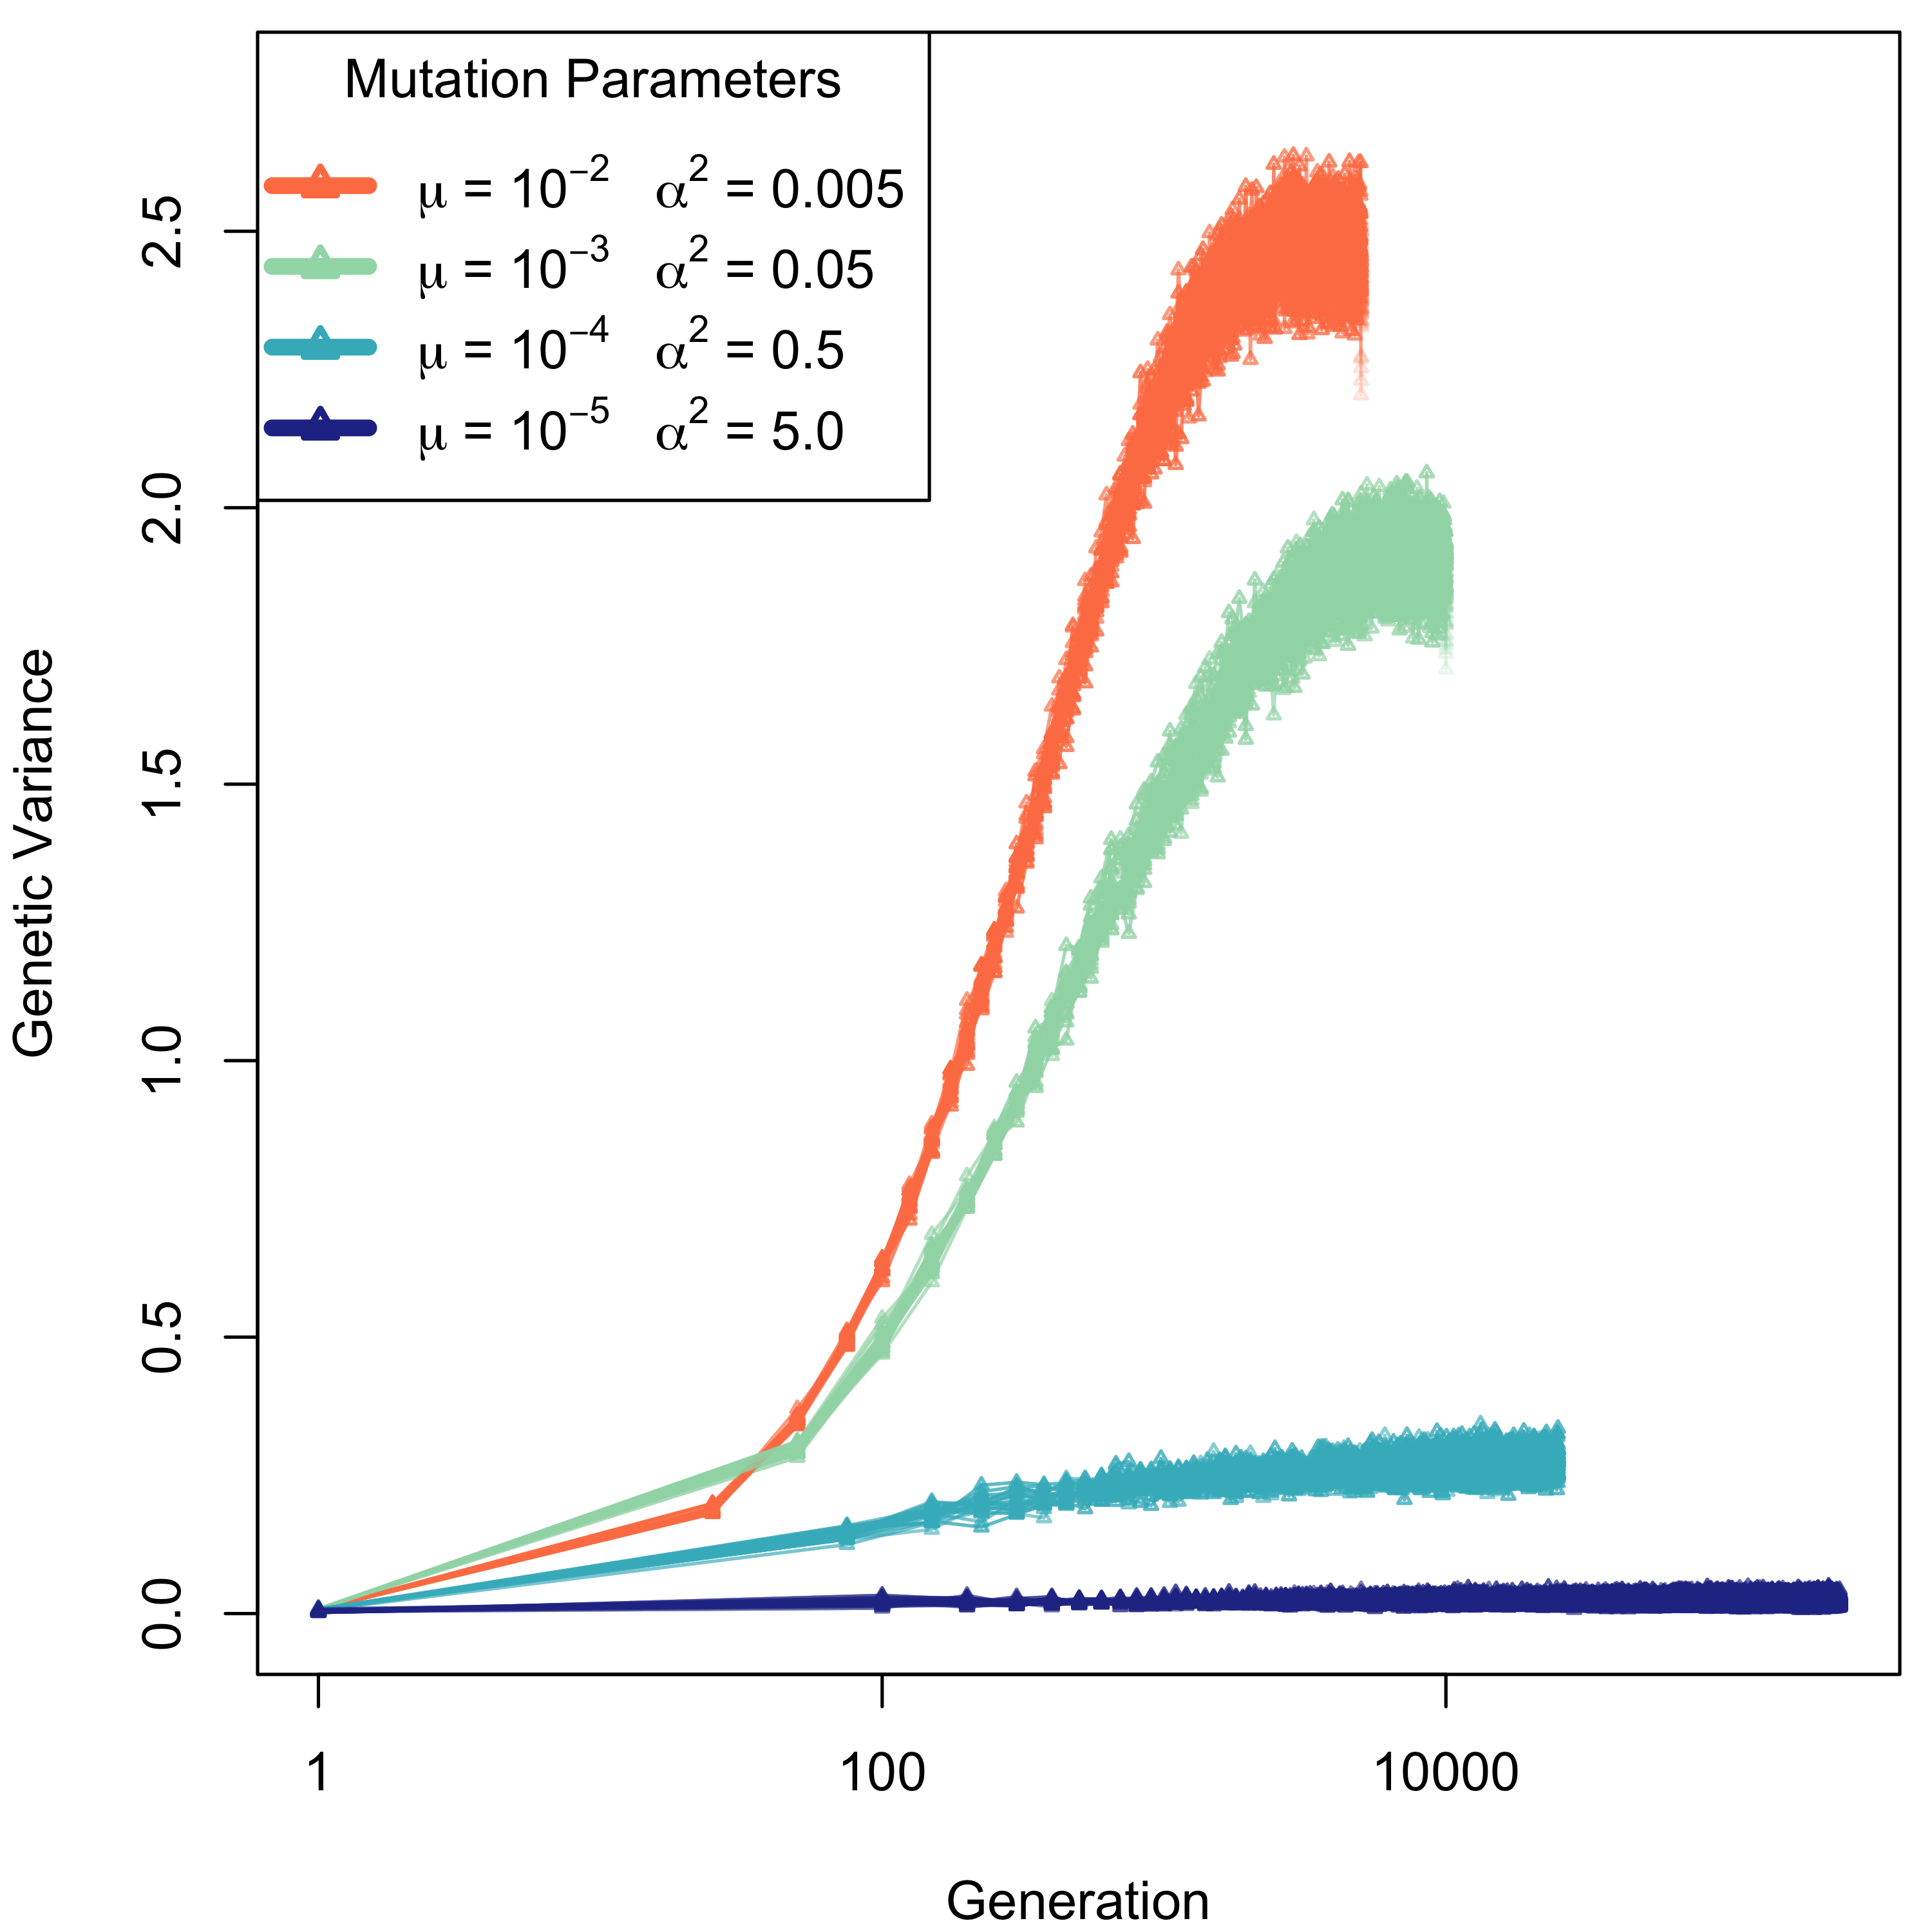
\includegraphics[width=0.9\linewidth]{Figures/CompareVa_OnePlot.png}}
\caption[Genetic variance across parameter sets.]{Genetic variance across parameter sets approaching respective equilibria during simulation burn-in.}
\label{fig:VaAmong}
\end{figure}


\begin{figure}[h]
\centering
\makebox[\textwidth]{
        \includegraphics[width=1\linewidth]{Figures/wait_times_200.pdf}}
\caption[~- Time spent before expansion into second patch.]{Time spent (in generations) before expansion into second patch for each genetic architecture regime with a larger dispersal kernel of $\sigma_{disperse} = 4$. Points are jittered for visualization. All points beyond the vertical dashed line are censored and did not expand during the course of the simulation.}
\label{fig:waittimes200}
\end{figure}


\begin{figure}[h]
\centering
\makebox[\textwidth]{
        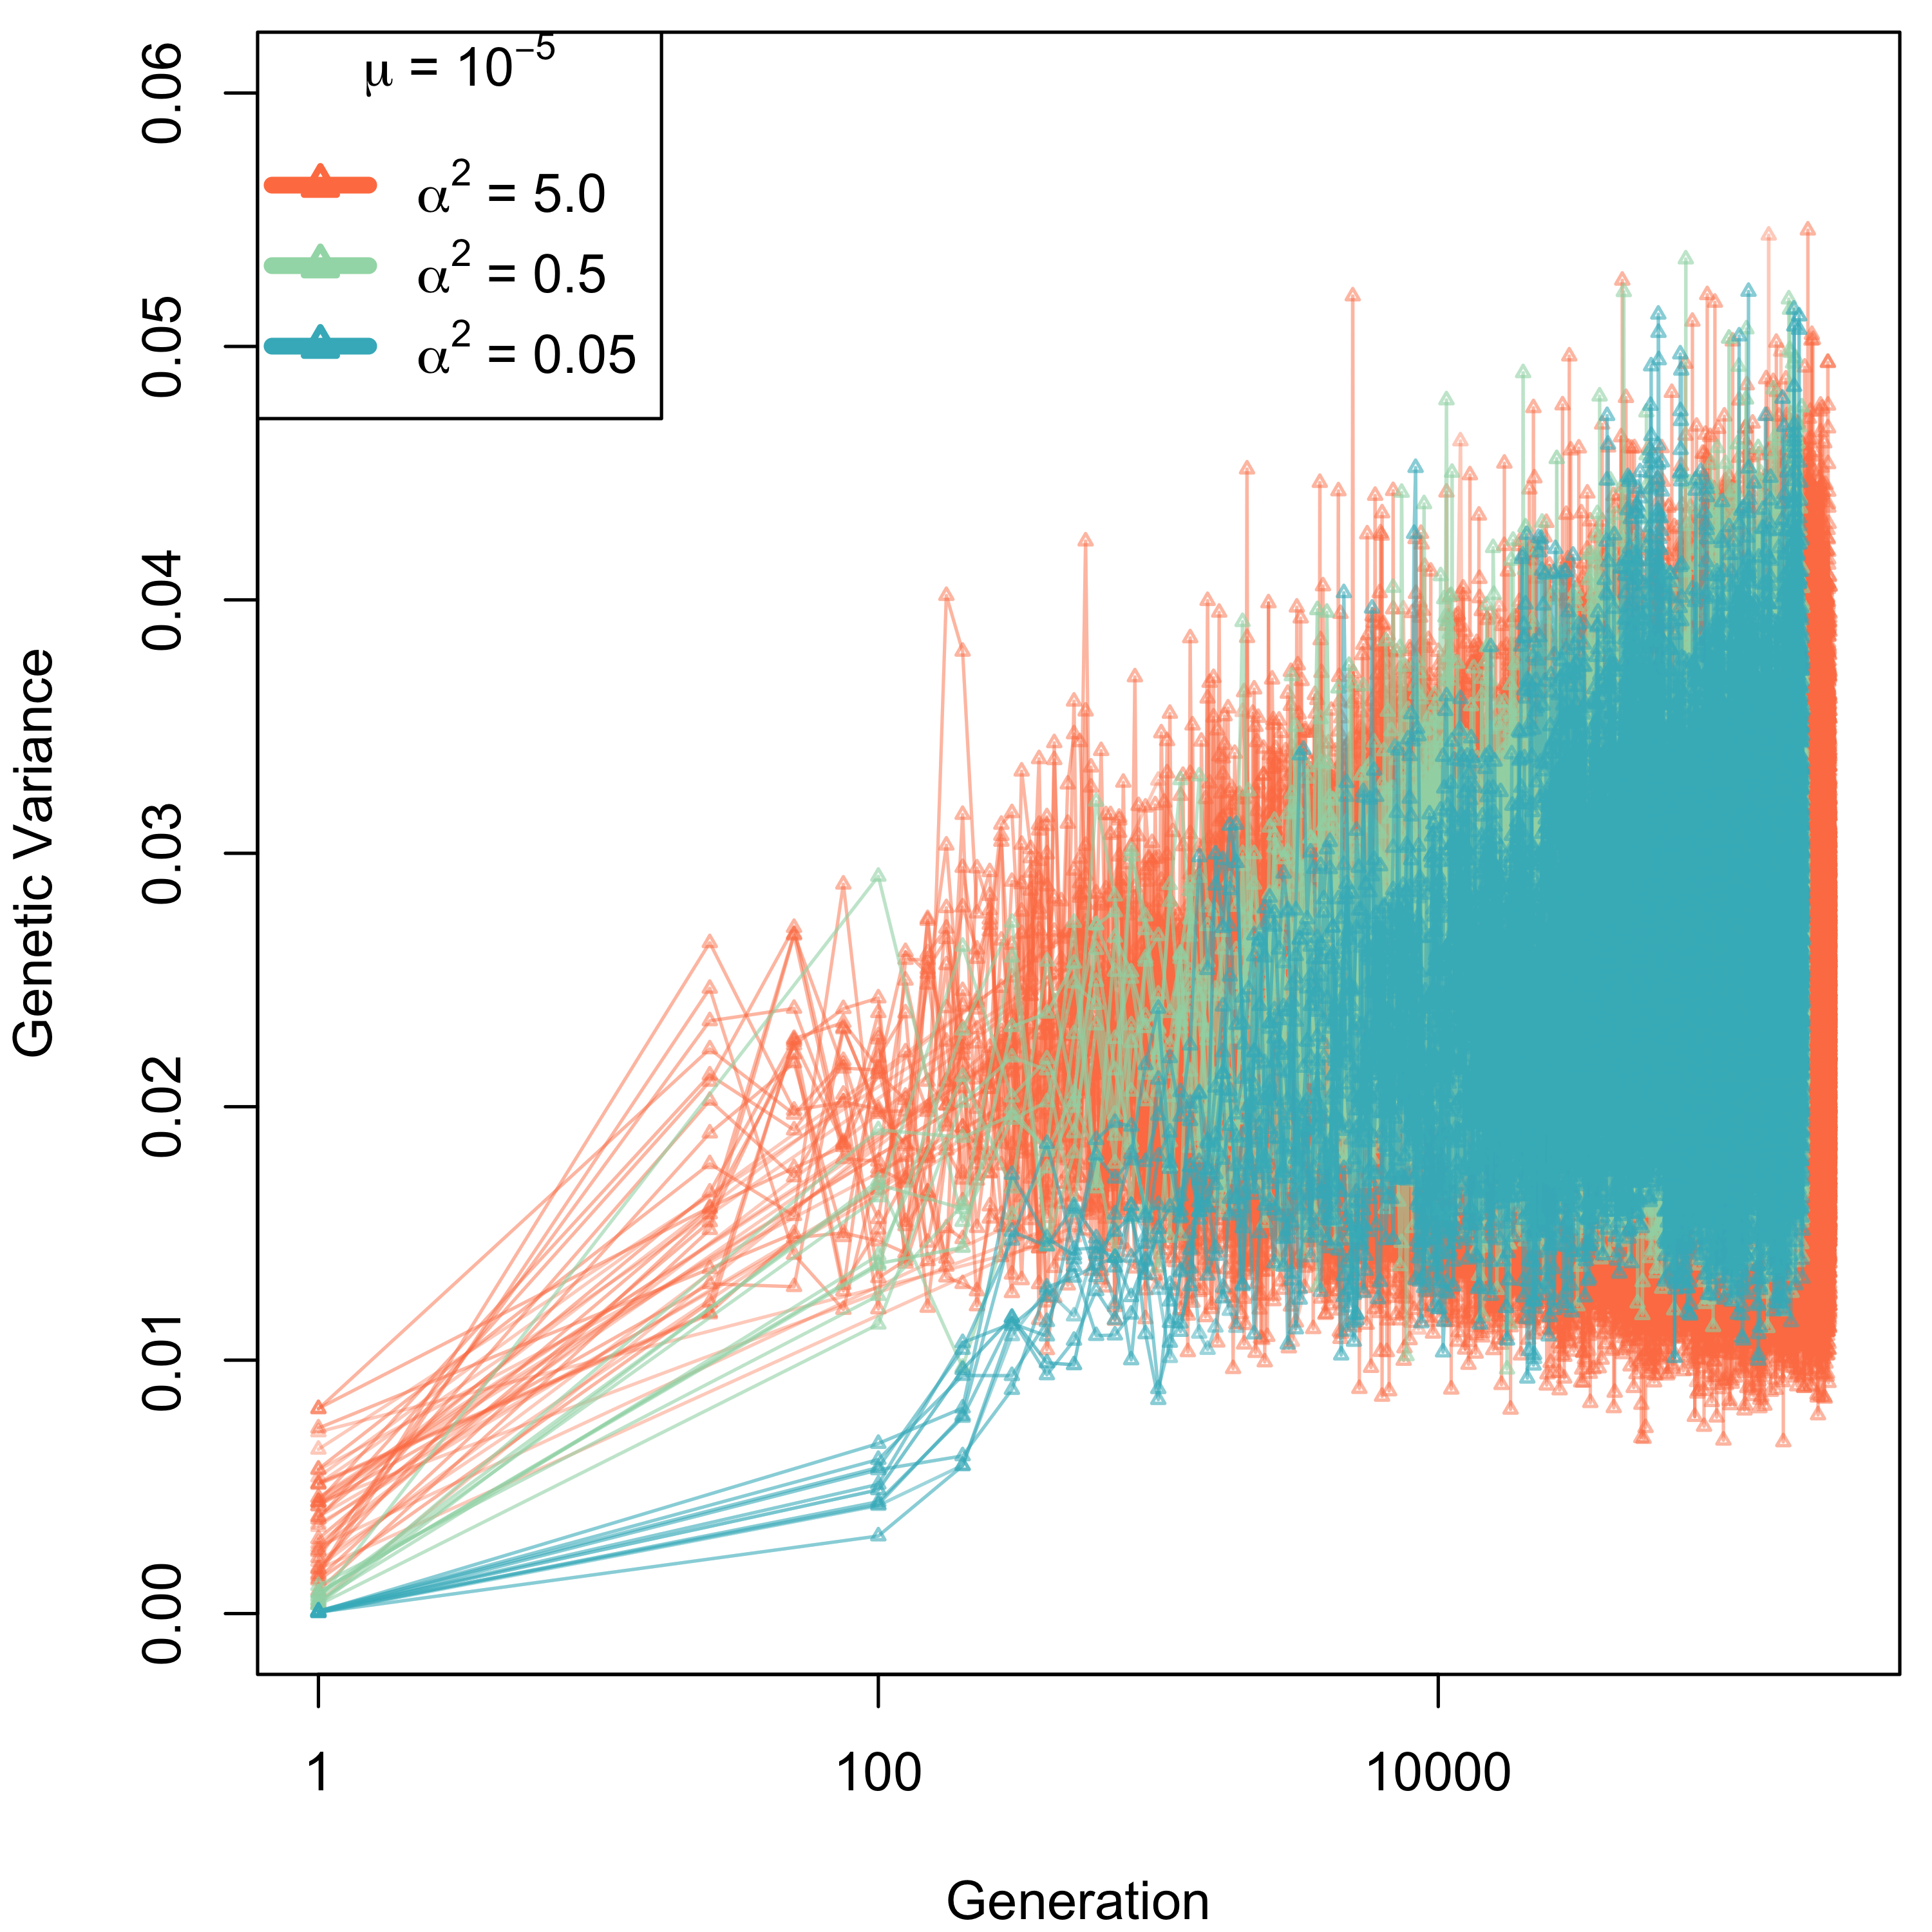
\includegraphics[width=0.9\linewidth]{Figures/constVg_CompareVa_OnePlot.png}}
\caption[Approximately constant genetic variance across parameter sets.]{Approximately constant genetic variance across parameter sets approaching respective equilibria during simulation burn-in.}
\label{fig:VaConst}
\end{figure}


%%% Local Variables:
%%% TeX-master: "thesis"
%%% TeX-PDF-mode: t
%%% End:
